%!TEX root = paper.tex

\section{The Common Fabric: Streaming Dataflows}
\label{sec:execution}

Although users can write Flink programs using a multitude of APIs, all Flink programs eventually compile down to a common representation: the dataflow graph\footnote{Internally called JobGraph}. The dataflow graph is executed by Flink's runtime engine, the common layer underneath both the batch processing (DataSet) and stream processing (DataStream) APIs.


\subsection{Dataflow Graphs}
The dataflow graph, as depicted in \autoref{fig:dataflow}, is a directed acyclic graph (DAG) that consists of (i) stateful operators, and (ii) data streams that represent data produced by an operator and are available for consumption by operators. Since dataflow graphs are executed in a data-parallel fashion, operators are parallelized into one or more parallel instances called \emph{subtasks} and streams are split into one or more \emph{stream partitions} (one partition per producing subtask).

\begin{figure}
\centering
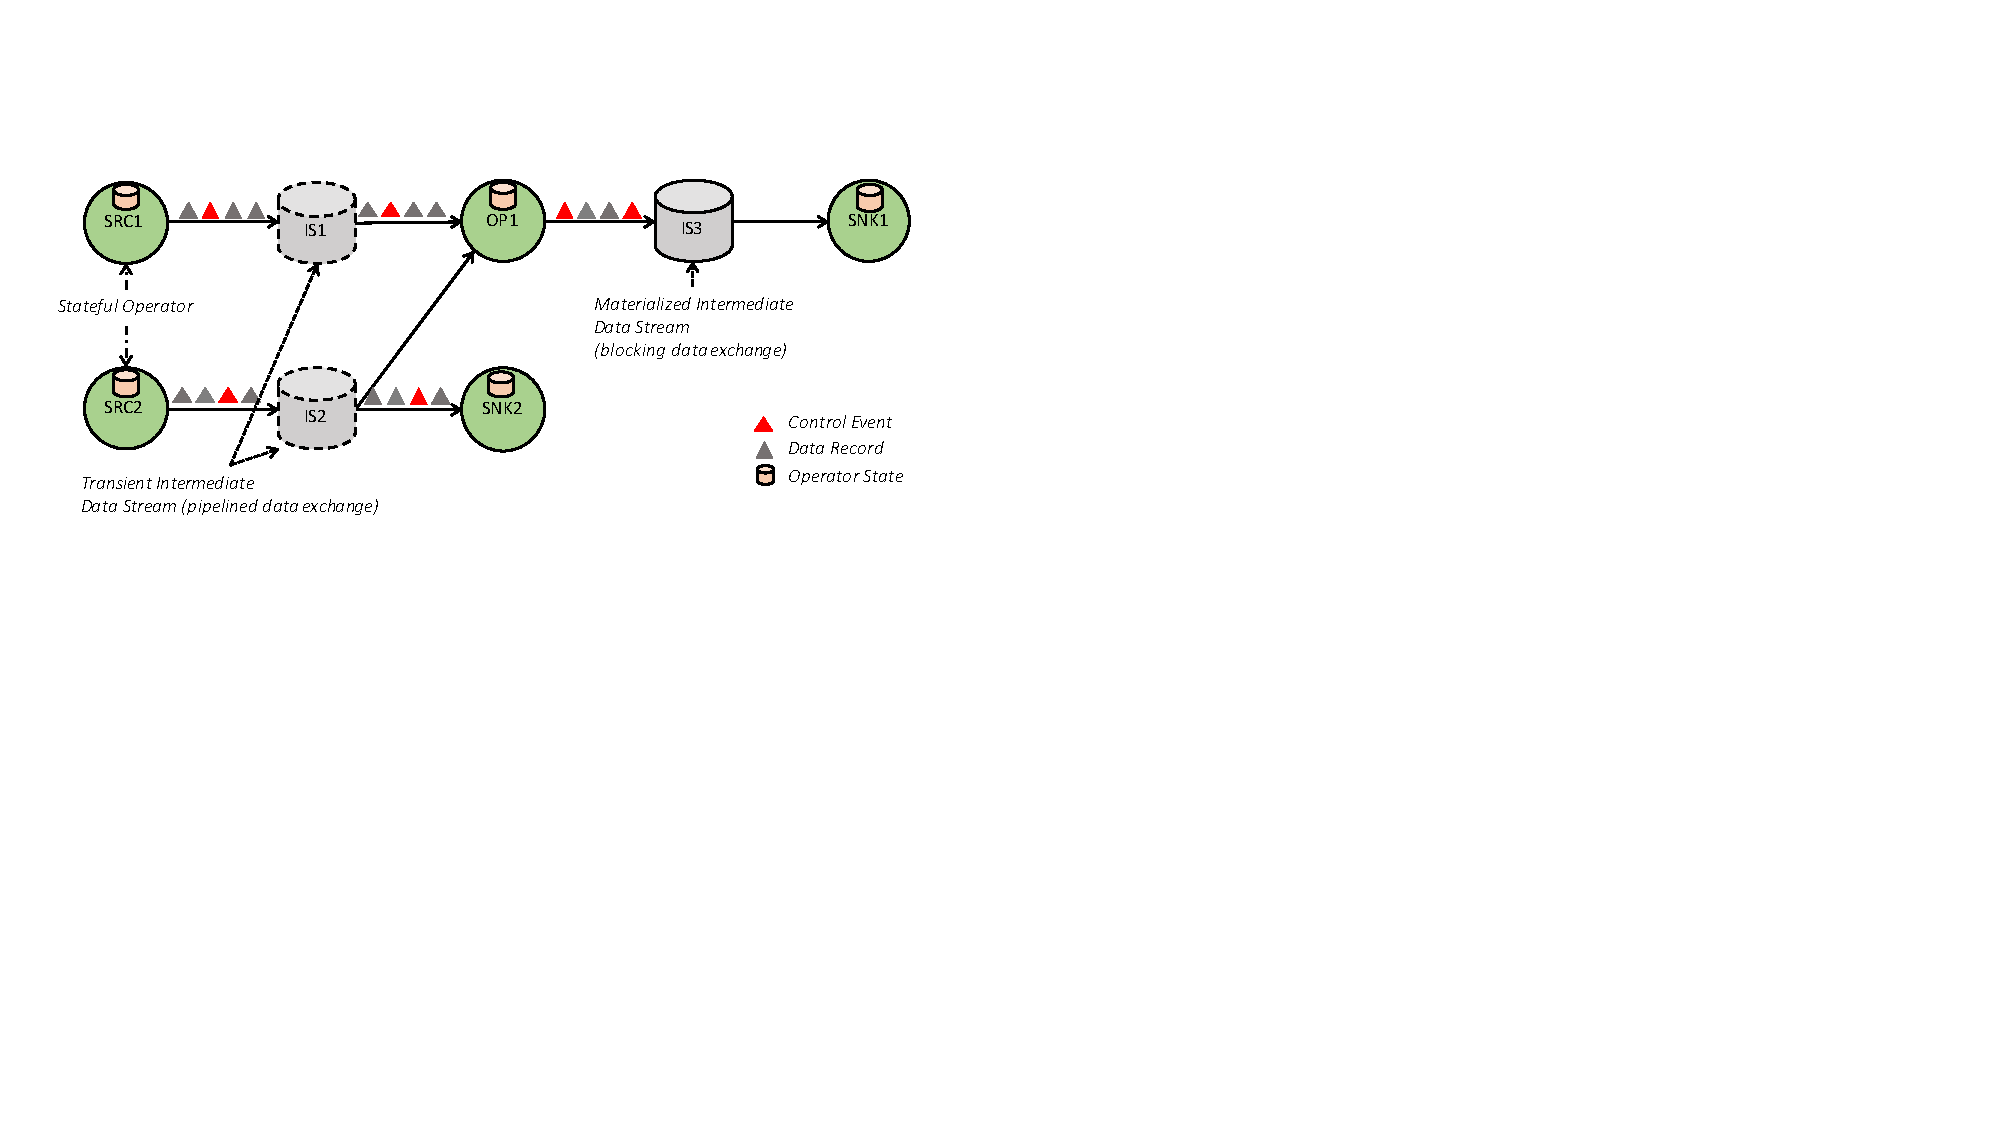
\includegraphics[width=.7\textwidth]{figs/dataflow}
\vspace{-3mm}
\caption{A simple dataflow graph comprising stateful operators (sources, sinks and operators), and intermediate streams (transient and materialized).}
\label{fig:dataflow}
\end{figure}


The stateful operators (which may be stateless as a special case) implement all processing logic, e.g., filters, hash joins, stream window functions, etc. Many of these operators are implementations of textbook versions of well known algorithms. \autoref{sec:streaming} provides details on the implementation of windowing operators. Streams distribute data between producing and consuming operators in various patterns, such as point-to-point, broadcast, re-partition, fan-out, or merge.


\subsection{Data Exchange through Intermediate Data Streams}
Flink's intermediate data streams are the core abstraction for data exchange between operators. The notion of intemediate data streams in Flink is broader than the traditional notion of a continuous transient stream. The particular behavior of a data stream is parameterized by the higher layers in Flink (e.g., the program optimizer used by the DataSet API). 


\para{Pipelined Data Exchange.} Pipelined streams exchange data between concurrently running producers and consumers resulting in pipelined execution. Synchronous streams propagate back pressure from consumer to producer (modulo some elasticity via intermediate buffer pools, in order to compensate for short-term throughput fluctuations). Flink uses these streams for continuous streaming programs, as well as for many parts of batch dataflows, in order to avoid materialization when possible.

\para{Blocking Data Exchange.} Blocking streams are applicable to bounded data streams. The decoupled stream buffers all of the producing operator's data before making it available for consumption, thereby separating the producing and consuming operators into different execution stages. Blocking streams naturally require more memory, frequently spill to secondary storage, and do not propagate backpressure. They are used to isolate successive operators against each other (where desired) and in situations where plans with pipeline-breaking operators such as joins, can cause distributed deadlocks.

\para{Balancing Latency and Throughput.} Flink’s data exchange mechanisms are implemented around the exchange of buffers. When a data record is ready on the producer side, it is serialized and stored into one or more buffers that can be forwarded to consumers. A buffer in Flink is sent to a consumer either i) as soon as it is full, or ii) when a timeout condition is reached. This enables Flink to achieve, high throughput by setting the size of buffers to a high value, e.g., a few kilobytes, as well as low latency by setting the buffer timeout to a low value e.g., a few milliseconds.

\para{Ordering Guarantees.} Data exchange of one stream partition preserves the order of records. As a consequence, chains of operators that consume one stream partition maintain order of records. Operators receiving more than one stream partition merge the streams as records arrive, to minimize back pressure. As a consequence, the streaming dataflow gives no ordering guarantees for records after any form of repartitioning or broadcasting. The responsibility to deal with out-of-order records is delegated to the operator implementation. We found that this gives the most efficient design, as most operators do not require deterministic order, and operators that need to compensate for out-of-order arrivals (such as event time windows) can do that efficiently.

\para{Control Events.} Apart from exchanging data, streams in Flink communicate different types of control events. These are special events injected in the data stream by producing operators and are delivered in-order along with all other data records and events within a stream partition. The receiving operators react to these events by performing certain actions upon their arrival. Flink uses control records in multiple mechanisms, such as: 
\begin{itemize}
\item Coordinating checkpoints, dividing the stream into pre-checkpoint and post-checkpoint (Section XCY)
\item To signal the progress of event time within a stream partition (Section XYZ). 
\item Bulk/Stale-Synchronous-Parallel iterative algorithms on top of cyclic dataflows, to signal that a stream partition has reached the end of a superstep.
\end{itemize}

\subsection{Iterative Dataflows}
{\color{red} Should we have a few sentences here? Would describe that cyclic flows enable iterative processing as BSP/SSP in batch [iterations paper, euranova SSP on Flink paper] and simply for streaming programs with feedback.}

Cycles are formed by special feedback streams. Feedback streams do not act as a dependency (not treated by the scheduler, so Flink keeps simple DAG scheduling techniques) and their contents is treated as operator state (simplifies fault tolerance). 

\subsection{Fault Tolerance}
Flink offers reliable execution with strict exactly-once-processing consistency guarantees and deals with failures via checkpointing and partial re-execution. The general assumption the system makes to effectively provide these guarantees is that the data sources are persistent and replayable. Examples of such sources are files and durable message queues (e.g. Apache Kafka). In practice, non-persistent sources can also be incorporated by keeping a look-ahead log within the state of the source operators. We provide more details about the approach we adopted to achieve fault tolerance for the DataSet and DataStream models respectively in sections 4.3 and 5.




































% \para{The Job Graph.} Flink's execution model is based on the Job Graph, a directed acyclic graph (DAG) that consists of nodes and edges. There are two classes of nodes: (stateful) operators, and (logical) intermediate results (IRs) as presented on Figure \autoref{fig:JobGraph}. For example, the aforementioned graph consists of five operators (circles), and three intermediate results (cylinders). Operators abstract computation (e.g., transformations, joins, etc), state (e.g., a persistent counter), as well as data sources (e.g. reading data from a file system, a socket, a message queue, etc.), and data sinks. Operators produce intermediate results, as well as updates to state. An intermediate result is a logical handle (pointer) to the data that is produced by one operator. An intermediate result can be consumed by one or more operators. Intermediate results are logical in the sense that the data they point to may or may not be materialized on disk. When the JobGraph is scheduled in a cluster for execution, it is parallelized to form an ExecutionGraph that consists of tasks (parallel instances of operators), and intermediate result partitions (IRPs).


% \para{Data Transfer.} The unit of data transfer in the Flink runtime is a buffer. Buffers contain one or more records, and a record can span multiple buffers. Buffers are requested and relinquished from local buffer pools, shared among operators that live in the same task manager. An IRP is simply a collection of buffers. Work in Flink progresses (i.e., records flow through the pipeline) as long as there are buffers available, essentially implementing distributed blocking queues (the logical streams) with bounded capacity (the amount of memory available to the buffer pools, which can be configured by the user). This mechanism, in addition to implementing record network transfers doubles down as a natural way to backpressure the flow in the case of slow operators (including external systems that consume data). 

% We mentioned that the intermediate results are logical handles to the data, rather than the data itself. Internally, intermediate results are abstract classes with many implementations. These implementations can perform pipelined data exchange, and blocking data exchange.

% \para{Pipelined Data Exchange.} Pipelining (also called intra-operator parallelism), means that a producing and a consuming operator make progress at the same time, without the consumer waiting for the producer to finish. Pipelining is required in streaming systems, and is also used in batch systems to reduce latency. Flink implements pipelining by implementing intermediate results which activate network transfers between the producer task and consumer task,  as soon as their first buffer is available. Flink allows the configuration of its buffers' size and timeout. A buffer is sent to its consumer task as soon it is filled,  or as soon as a timeout is reached. Hence, by setting the buffer size and/or timeout to lower values, one can reduce latency, while achieving the opposite effect (i.e., high throughput) by using higher values.

% \para{Blocking Data Exchange.} Sometimes it is desirable to break a job into stages, scheduling and executing each stage individually (e.g., to enable interactive processing, and better staging of resources in large batch jobs). To do that, the system has to materialize intermediate results (in memory or disk). Flink implements blocking data exchange via an intermediate result that signals its availability only when all the buffers from the producer have been materialized. The cached buffers can double down as a materialized reusable intermediate result. 

